\clearpage
\chapter[RESULTS, ANALYSIS AND DISCUSSION]{Results, Analysis and Discussion}
\label{ch:results}

\section{Results}\label{sec:resultsmain}

\subsection{A change of workload is not a fault: the ML correction}
\label{sec:workloadres}
The first ML engine judged each service with two Isolation Forests fitted on that service's recent readings. On the benchmark faults it looked fine, but an operator who stopped the traffic generator and switched to the ML engine saw every service with an anomaly score of 100\%. We reproduced it on recordings made for the purpose. Both benches ran live in Docker, reached by the mapper over SSH, with \emph{no fault at all}; only the work changed (\code{run/scripts/workload-shift-experiment.sh} and \code{workload-steps-experiment.sh}). In the first pair of recordings (two benches, 62 minutes) the organic traffic generator ran, stopped, ran, stopped longer and ran again. In the second pair (two benches, 72 minutes) a closed-loop generator held a constant number of visitors and stepped it $2 \to 8 \to 2 \to 0 \to 20 \to 2$, which moved the entry service's network traffic between 0 and about $3 \times 10^{5}$\,B/s (Figure~\ref{fig:workload}a). Every alarm in these recordings is a false alarm by construction.

The forest was in alarm for 23\% of the organic recording and for 52\% of the steady-load recording (Figure~\ref{fig:workload}b, Table~\ref{tab:models}). The other workload-blind detectors do the same or worse, from 38\% to 75\% on the organic recording and from 76\% to 96\% on the steady one, because all of them model the readings themselves and a new workload is outside what they were fitted on. It is not a tuning matter. A forest scores a value beyond its training range no higher than its most extreme training point, so the old engine had added a range guard. That guard fires at once for every service when the traffic changes for all of them, and a large shift needed thirty minutes to be accepted as the new normal. On the fault-free stretches of the live fault campaigns the same engine raised 40.9 alarm episodes per hour.

The corrected engine (Section~\ref{sec:load}) does not alarm on either recording (0\% and 0\% of the time; one false episode in 72 minutes of steady-load steps, none in 62 minutes of organic traffic). Figure~\ref{fig:workload}c shows the load factor it read: it follows the steps of Figure~\ref{fig:workload}a. It rises to about $+2$ at the twenty-visitor step (traffic about seven times the reference) and falls to about $-1.2$ when the traffic stops (the log scale saturates at the network unit). That is how the shift gets explained instead of judged. The model finds the change by itself: no setting names the load generator, and nothing is installed on the hosts.

\begin{figure}[!htbp]
\centering
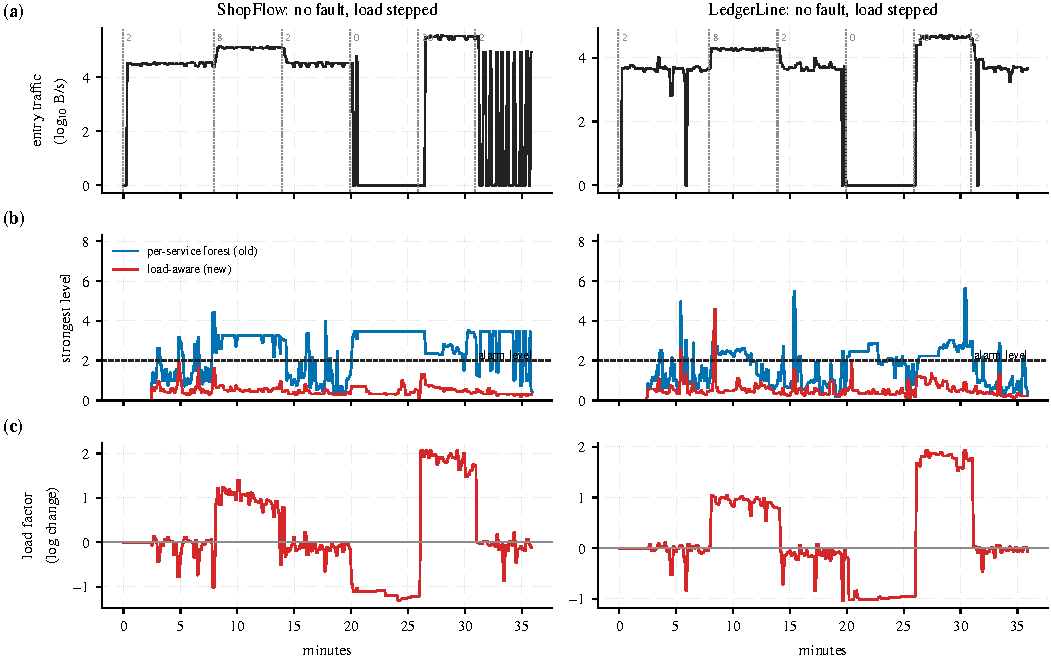
\includegraphics[width=\textwidth]{fig_workload.pdf}
\caption[Fault-free recordings with the load stepped]{Two fault-free recordings with the load stepped (left ShopFlow, right LedgerLine; dotted lines mark a new level of concurrent visitors). (a) Network traffic into the entry service. (b) The strongest service level of the old per-service forest and of the load-aware model; the dashed line is the alarm level. (c) The load factor $L(t)$ the new model read, as a logarithmic change from its reference.}
\label{fig:workload}
\end{figure}

\subsection{Which model of normal}
\label{sec:whichmodel}
Every candidate of Section~\ref{sec:candidates} runs inside the same engine and is judged on four kinds of recording (Table~\ref{tab:models}, Figure~\ref{fig:models}): the 62 real faults, the 84 faults of the live Fault Lab campaigns (Section~\ref{sec:live}), 125 synthetic faults, and the two fault-free workload recordings. The replay feeds every recorded moment to the engine as one reading, as the live server does; the earlier replay dropped consecutive identical readings, which removed the idle stretches from the data (Section~\ref{sec:bug2}).

\begin{table}[!htbp]
\centering
\caption[Models of normal compared on faults and on workload shifts]{Models of normal compared inside the same engine. For each set of injected faults: share of faults caught with the true cause first (\cn, \%) and false-alarm episodes per fault-free hour. Last two columns: share of the time in alarm in the fault-free recordings of organic traffic and of steady-load steps (\%); every alarm there is false.}
\label{tab:models}
\scriptsize
\setlength{\tabcolsep}{3pt}
\begin{tabular}{lrrrrrrrr}
\toprule
 & \multicolumn{2}{c}{Real (62)} & \multicolumn{2}{c}{Live (84)} & \multicolumn{2}{c}{Synthetic (125)} & \multicolumn{2}{c}{No faults, load moves}\\
Model & \cn & FA/h & \cn & FA/h & \cn & FA/h & organic & steps\\
\midrule
Rule engine (z-score, no model) & 63 & 9.2 & 45 & 16.3 & 75 & 2.6 & 12 & 35 \\
\midrule
Isolation Forest (old default) & 69 & 4.6 & 46 & 40.9 & 76 & 0.2 & 23 & 52 \\
Ensemble of four detectors & 71 & 20.0 & 44 & 81.7 & 78 & 2.6 & 47 & 88 \\
k-NN & 69 & 13.8 & 44 & 57.2 & 72 & 5.2 & 73 & 96 \\
Mahalanobis & 71 & 23.8 & 45 & 65.4 & 84 & 2.6 & 38 & 76 \\
HBOS & 69 & 34.6 & 44 & 57.2 & 77 & 1.4 & 75 & 82 \\
Control chart, MAD spread & 73 & 10.0 & 44 & 24.5 & 79 & 0.6 & 13 & 31 \\
Control chart, tail spread & 71 & 2.3 & 46 & 0.0 & 78 & 0.2 & 0 & 0 \\
Subspace residual, 1 component & 68 & 3.1 & 50 & 8.2 & 78 & 0.4 & 1 & 3 \\
Subspace residual, 2 components & 68 & 3.8 & 50 & 0.0 & 77 & 0.2 & 1 & 4 \\
Load factor, MAD spread & 71 & 3.8 & 43 & 16.3 & 79 & 0.6 & 10 & 6 \\
\textbf{Load factor, tail spread (adopted)} & 71 & 2.3 & 48 & 0.0 & 78 & 0.2 & 0 & 0 \\
\bottomrule
\end{tabular}
\end{table}

\begin{figure}[!htbp]
\centering
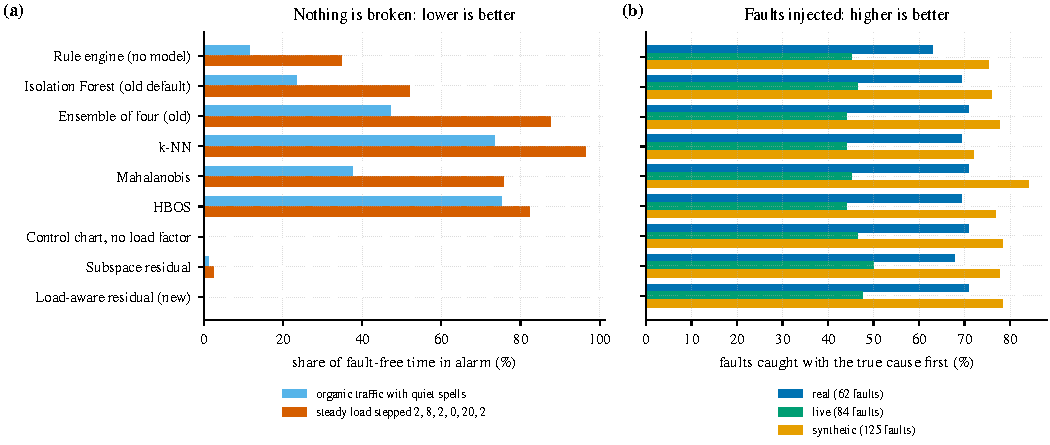
\includegraphics[width=\textwidth]{fig_models.pdf}
\caption[The candidate models on fault-free workload shifts and on injected faults]{The candidate models. (a) Share of fault-free time in alarm on the two workload recordings (lower is better). (b) Share of injected faults caught with the true cause first on the real, live and synthetic sets (higher is better).}
\label{fig:models}
\end{figure}

\begin{enumerate}
\item On injected faults the models are alike. The caught-and-named rate is $68$--$73\%$ on the real faults, $43$--$50\%$ on the live ones and $72$--$84\%$ on the synthetic ones for every candidate; differences of a few points are inside the noise of 62 to 125 faults (the intervals of Table~\ref{tab:main} are $\pm 10$ points). The workload-blind models differ in false alarms: the forest-family detectors raise 4.6 to 34.6 episodes per hour on the real systems and 40.9 to 81.7 on the live ones, against 2.3 and 0.0 for the adopted model.
\item On workload shifts they are not alike. The adopted model is in alarm for 0\% of both recordings; the workload-blind family for 23--75\% and 52--96\%. Replacing the forests by a robust residual with the tail-aware spread is the larger part of the improvement (control chart: 0\% and 0\%); the MAD spread alone is not enough (13\% and 31\%), because it treats bursty signals as Gaussian.
\item The load factor removes what is left. The control chart without it still raises 1.2 and 1.9 false episodes per hour on the two recordings; with it 0.0 and 1.0, and it is the better of the two on the live faults (47.6\% against 46.4\% caught and named). The subspace residual is the strongest alternative (3\% and 4\% of the steady recording in alarm; 50\% caught and named on the live faults). It raises 7.7 to 10.7 false episodes per hour on the steady steps, is slower to adapt, and its cost grows faster than linearly (Section~\ref{sec:cost}).
\end{enumerate}
We therefore adopted the load factor with the tail spread. We report what it does not do: it is not more accurate than the forest on the injected faults (71\% against 69\% on the real ones, inside the noise). A fault that begins during a large change of load can also be masked, because the model then accepts a deviation that either hypothesis about the load explains. Brownouts of nearly idle services remain the open problem for every model (no signal moves), as in the earlier version.

\paragraph{Sensitivity.} Figure~\ref{fig:zline} sweeps the alarm line. A looser line (2 spreads) raises detection to 94\% on the real faults but also the false alarms on the workload recordings (15.0 episodes per hour); a tighter one (6 or 8 spreads) removes all false alarms on the workload recordings but loses detection (87\% and 85\% on the real faults, 83\% and 75\% on the synthetic ones). The adopted line of 4 spreads is the loosest that keeps the workload recordings quiet. The training window (60, 120 or 240 readings) and the slow reference (120, 360 or 720) matter little once they are long enough; a window of 60 readings makes the workload recordings noisy again (10.4 false episodes per hour). We also tried carrying the range guard of the first model over to the residual (a value several floors beyond everything in the window counts as level one): it changed no result on any set of injected faults and added false alarms on the steady-load steps (4.8 episodes per hour at four floors, 1.0 without it), so the adopted model has none.

\paragraph{How fast a mild shift becomes normal.} A deviation that stays between level one and three is accepted as the new normal after $24$ readings (two minutes). Waiting longer, $48$ to $240$ readings, changed nothing on the injected faults (\cn{} $71\%$ on the real ones and $78\%$ on the synthetic ones at every value; synthetic detection $88\%$ against $89$--$90\%$) and nothing on the workload recordings, but doubled the time in alarm on the real systems ($6\%$ to $13\%$) and raised their false alarms from $2.3$ to $3.1$ per hour, because a service whose footprint changes after a restart stays in alarm until it is accepted. The cost of the short setting is that a slow fault that stays only mildly above the line is absorbed after two minutes, as in the simulated slow \texttt{payment} of Section~\ref{sec:engineslive}; a larger shift (level three or more) still needs thirty minutes.

\begin{figure}[!htbp]
\centering
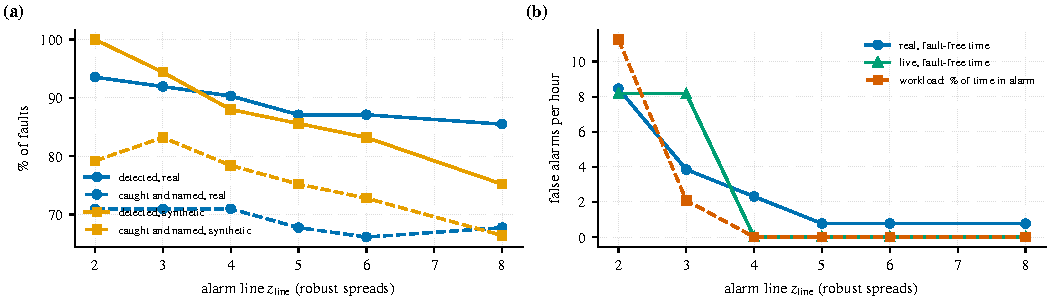
\includegraphics[width=\textwidth]{fig_zline.pdf}
\caption[Sensitivity of the adopted model to its alarm line]{Sensitivity of the load-aware model to its alarm line $z_{\mathrm{line}}$ (the engine alarms at level 2, that is, at $2 z_{\mathrm{line}}$ spreads). (a) Faults detected, and caught and named, on the real and synthetic sets. (b) False alarms per fault-free hour on the real and live sets, and the share of time in alarm on the workload recordings.}
\label{fig:zline}
\end{figure}

\subsection{Rules, the old ML and the new ML side by side}
\label{sec:threeway}
Table~\ref{tab:threeway} puts the three engines a user can pick in the top bar next to each other. The same harness replays them over the same recordings: the rule engine (robust z-score per metric, alarm at three spreads, no model), the first ML engine (per-service Isolation Forests) and the corrected ML engine (load-aware residual). Both ML engines name the source with the same random walk, so any difference between them comes from the model of normal. A longer version with the reasoning in plain words is kept in the repository as \code{wiki/44-ml-comparison.md}.

\begin{table}[!htbp]
\centering
\caption[Rules, old ML and new ML on the same recordings]{The three engines on the same recordings. \cn: faults caught with the true cause named first (\%). FA/h: false-alarm episodes per fault-free hour. Workload columns: share of the fault-free workload recordings spent in alarm (\%). ROC: per-reading AUROC and average precision on the real run and the held-out synthetic set. Cost: mean milliseconds per decision window for 10 and 320 services.}
\label{tab:threeway}
\footnotesize
\setlength{\tabcolsep}{4pt}
\begin{tabular}{lrrr}
\toprule
 & Rules & Old ML (forest) & New ML (load-aware)\\
\midrule
\multicolumn{4}{l}{\emph{Injected faults}}\\
Real, 62 faults: \cn{} / FA/h & 63\% / 9.2 & 69\% / 4.6 & \textbf{71\% / 2.3}\\
Live, 84 faults: \cn{} / FA/h & 45\% / 16.3 & 46\% / 40.9 & \textbf{48\% / 0.0}\\
Synthetic, 125 faults: \cn{} / FA/h & 75\% / 2.6 & 76\% / 0.2 & \textbf{78\% / 0.2}\\
Detected, real / live / synthetic & 90\% / 96\% / 83\% & 87\% / 99\% / 87\% & 90\% / 99\% / 88\%\\
Median delay, real & 15 s & 12 s & 12 s\\
\midrule
\multicolumn{4}{l}{\emph{No fault, only the workload moves}}\\
Organic on/off: time in alarm & 12\% & 23\% & \textbf{0\%}\\
Steps 2--8--2--0--20--2: time in alarm & 35\% & 52\% & \textbf{0\%}\\
\midrule
\multicolumn{4}{l}{\emph{Per-reading ranking}}\\
AUROC / AP, real & 0.69 / 0.34 & 0.63 / 0.29 & 0.66 / 0.31\\
AUROC / AP, synthetic test & 0.87 / 0.67 & 0.86 / 0.53 & 0.84 / 0.66\\
\midrule
Cost, 10 / 320 services (ms) & -- & 8.9 / 296 & 4.0 / 119\\
\bottomrule
\end{tabular}
\end{table}

The table reads in three parts. On injected faults the rule engine catches about as many faults as the ML engines. With container facts ranked first it names the right service for 63\% of the real faults, against 69\% for the old ML and 71\% for the new one. It also raises four times as many false alarms as the new engine on the real run and more than ten times as many on the synthetic set. Every swing of traffic is a deviation to it, and when no container fact is present the loudest service, often a victim, gets the blame. The two ML engines are close on the injected faults; the new one is two points ahead on each set, with fewer false alarms, mostly on the live campaigns, where restarts and traffic pauses are frequent. On the workload recordings the difference is the whole point of the correction: the old ML is in alarm for about half of the steady-load recording, the rule engine for a third of it, and the new ML not at all. Per reading, the rule z-score ranks best on both sets; a single high reading is cheap, and the rule engine loses only once alarms need persistence and a named source. Between the ML engines, the new one has the higher average precision on the held-out set and a slightly lower AUROC, and it is the cheaper of the two.

The new engine differs from the old one in five ways. Before judging any service, it estimates how much the whole project's workload moved and explains that move away. A fault during a load change still shows, because the load is a median that one or two services cannot drag, and a signal counts as normal only if it either ignores the load or follows it. Bursty signals get a fair spread, the engine never learns from readings it alarmed on, and each alarm says which signal moved and by how much. The rules the mapper was built on stay: no labels, no agent on the hosts, only the telemetry the mapper already reads.

\subsection{Detection and root cause}
Table~\ref{tab:main} compares the engines in one harness, now with the corrected ML engine inside. On the real systems the hybrid and the ML engine name the true cause first for 71\% of all faults, against 63\% for the rule layer and 68\% for ranking by anomaly alone. The paired differences are in Figure~\ref{fig:forest}. They are smaller than in the first version of this report and no longer reach significance. Hybrid over rules is $+8.1$ points on the real systems (95\% CI $[-1.6, +17.7]$, $p = 0.117$) and $+5.6$ on the synthetic set ($[-0.6, +11.8]$, $p = 0.093$). Hybrid over the severity ranking is $+3.2$ and $+1.1$ points, and hybrid over the ML engine $0.0$ and $+0.6$. With 62 real faults a difference below about ten points cannot be resolved. What the corrected engine changes is the false-alarm column: the ML engine alarms 2.3 times per fault-free hour on the real systems and 0.2 on the synthetic set, the quietest row, and Section~\ref{sec:workloadres} shows that it stays quiet when only the load moves. The hybrid raises more episodes (6.2 and 0.9) because the rule layer may also trigger it.

\begin{table}[!htbp]
\centering
\caption[Detection and root cause in one harness (point estimates with 95\% bootstrap intervals over faults)]{Detection and root cause in one harness (point estimates with 95\% bootstrap intervals over faults). Det.: faults detected (\%). \acc{1}, \acc{3}: true cause first or in the top three among detected (\%). \cn: caught and named first over all faults (\%). FA/h: false-alarm episodes per fault-free hour. Alarm: share of fault-free time in alarm (\%).}
\label{tab:main}
\footnotesize
\setlength{\tabcolsep}{3pt}
\begin{tabular}{lcccccc}
\toprule
Engine & Det. [95\% CI] & \acc{1} & \acc{3} & \cn{} [95\% CI] & FA/h & Alarm \\
\midrule
\textit{Real benches (62 faults, 217 min)} & & & & & & \\
Rules & 90 [82, 97] & 70 & 91 & 63 [52, 74] & 9.2 & 9 \\
Severity ranking & 90 [82, 97] & 75 & 86 & 68 [56, 79] & 6.2 & 8 \\
ML engine & 90 [82, 97] & 79 & 89 & 71 [60, 81] & 2.3 & 6 \\
\textbf{Hybrid} & 90 [82, 97] & 79 & 89 & 71 [60, 81] & 6.2 & 8 \\
Hybrid + change-point & 95 [89, 100] & 76 & 88 & 73 [61, 82] & 5.4 & 16 \\
Hybrid + learned dir. & 90 [82, 97] & 75 & 89 & 68 [55, 77] & 6.2 & 8 \\
\midrule
\textit{Synthetic held-out (178 faults, 16 topologies)} & & & & & & \\
Rules & 89 [84, 93] & 78 & 95 & 70 [62, 76] & 2.5 & 2 \\
Severity ranking & 93 [89, 97] & 80 & 92 & 74 [67, 80] & 0.9 & 5 \\
ML engine & 92 [87, 96] & 82 & 94 & 75 [69, 81] & 0.2 & 4 \\
\textbf{Hybrid} & 93 [89, 97] & 81 & 93 & 75 [69, 81] & 0.9 & 5 \\
Hybrid + change-point & 94 [90, 98] & 80 & 92 & 75 [69, 81] & 0.8 & 6 \\
Hybrid + learned dir. & 93 [89, 97] & 81 & 93 & 75 [69, 81] & 0.9 & 5 \\
\bottomrule
\end{tabular}
\end{table}

The operating curves (Figure~\ref{fig:op}) show why the comparison is delicate. The engines trade detection for false alarms along nearly overlapping curves. The hybrid and the ML engine sit on or near the upper envelope in both sets, above the rules at almost every false-alarm budget, so their advantage lies in the operating point and not in a single threshold. Figure~\ref{fig:class} breaks C+N down by fault class. The gain over the rules is concentrated in stop faults (16 of 16 against 9 of 16 on the real systems), which is the effect of the \texttt{docker stop} fact, and, on the synthetic set, in flap faults (12 of 12 against 2 of 12).

\begin{figure}[!htbp]
\centering
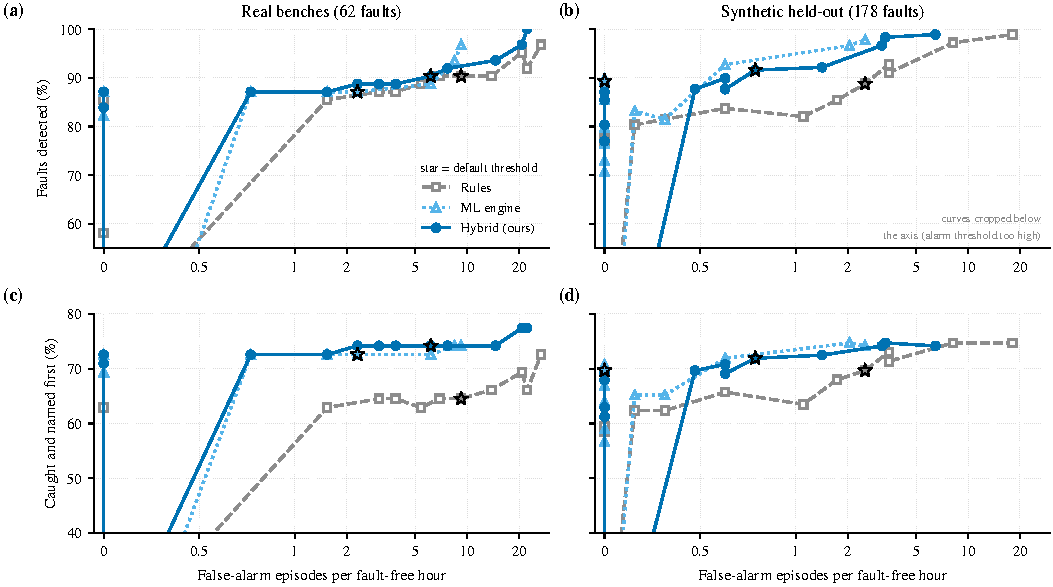
\includegraphics[width=\textwidth]{fig_op.pdf}
\caption[Operating curves. Sweeping the alarm threshold of each engine traces detection rate]{Operating curves. Sweeping the alarm threshold of each engine traces detection rate (top) and caught-and-named rate (bottom) against false-alarm episodes per fault-free hour (symmetric-log axis); stars mark the default threshold. The hybrid sits on the upper envelope in both the real systems (a, c) and the synthetic held-out set (b, d).}
\label{fig:op}
\end{figure}

\begin{figure}[!htbp]
\centering
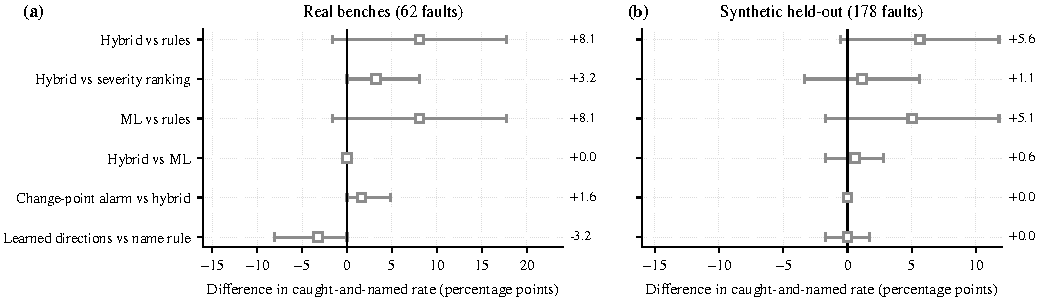
\includegraphics[width=\textwidth]{fig_forest.pdf}
\caption[Paired differences in caught-and-named rate between engines]{Paired differences in caught-and-named rate between engines (percentage points, 95\% paired-bootstrap interval); filled markers exclude zero.}
\label{fig:forest}
\end{figure}

\begin{figure}[!htbp]
\centering
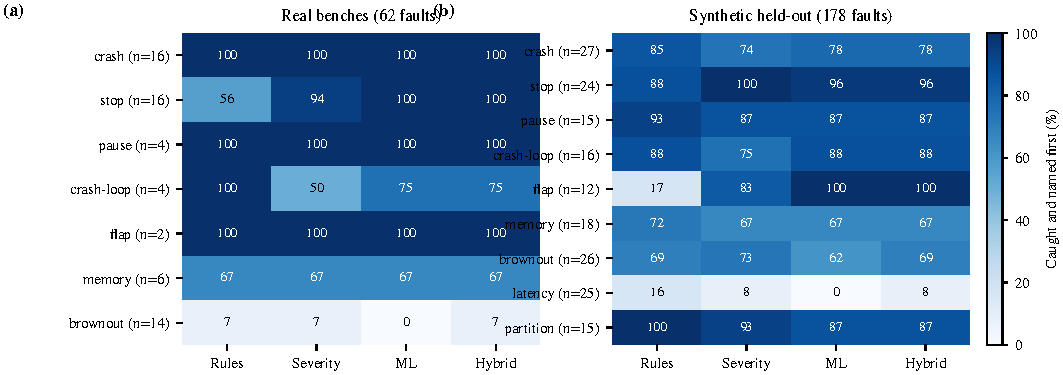
\includegraphics[width=\textwidth]{fig_class.pdf}
\caption[Caught-and-named rate by fault class]{Caught-and-named rate by fault class (percent; $n$ faults per class), for four rankers on the real systems (a) and the synthetic held-out set (b). Brownouts are the open problem on the real systems.}
\label{fig:class}
\end{figure}

\subsection{Which detector}
Table~\ref{tab:roc} scores each model of normal as a service-level classifier, now including the control chart, the subspace residual and the adopted load-aware model. As before, the plain rule $z$-score is as good as or better than every learned detector at separating a faulted service from a healthy one by AUROC (0.695 against 0.629 for the old forest and 0.665 for the load-aware model on the real systems; 0.873 against 0.862 and 0.842 on the synthetic set). On average precision, which weighs the rare faulted services, the load-aware model is above every forest-family detector on both sets (0.313 against at most 0.290 on the real systems; 0.665 against at most 0.608 on the synthetic set). It is level with the rules on the synthetic set (0.666). Separation on the real systems is weak for every detector (AUROC 0.62 to 0.70), because many real faults hit services that are nearly idle.

Discrimination is therefore not what chose the model; behaviour under a change of workload was (Section~\ref{sec:whichmodel}). The adopted model is quiet (alarm time of 6\% against 9\% for the rules on the real systems, Table~\ref{tab:main}); it separates own from symptom evidence; and its alarms complement those of the rules, so their union detects more faults than either on the synthetic set (93\% against 89\%).

\begin{table}[!htbp]
\centering
\caption[Service-level detection by detector (mean $\pm$ s.d]{Service-level detection by model of normal (mean $\pm$ s.d. over three seeds for the randomised detectors; the rule layer and the three residual models are deterministic).}
\label{tab:roc}
\footnotesize
\begin{tabular}{lcccc}
\toprule
 & \multicolumn{2}{c}{Real} & \multicolumn{2}{c}{Synthetic} \\
Detector & AUROC & AP & AUROC & AP \\
\midrule
Rule z-score & 0.695$\pm$0.000 & 0.337$\pm$0.000 & 0.873$\pm$0.000 & 0.666$\pm$0.000 \\
Isolation Forest (old) & 0.629$\pm$0.004 & 0.288$\pm$0.003 & 0.862$\pm$0.004 & 0.528$\pm$0.020 \\
k-NN & 0.668$\pm$0.010 & 0.193$\pm$0.004 & 0.860$\pm$0.001 & 0.517$\pm$0.004 \\
Mahalanobis & 0.650$\pm$0.003 & 0.290$\pm$0.004 & 0.868$\pm$0.001 & 0.608$\pm$0.006 \\
HBOS & 0.620$\pm$0.005 & 0.274$\pm$0.006 & 0.853$\pm$0.004 & 0.473$\pm$0.030 \\
Ensemble of four & 0.650$\pm$0.006 & 0.287$\pm$0.009 & 0.865$\pm$0.001 & 0.593$\pm$0.002 \\
Control chart (no load factor) & 0.669$\pm$0.000 & 0.302$\pm$0.000 & 0.842$\pm$0.000 & 0.657$\pm$0.000 \\
Subspace residual & 0.696$\pm$0.000 & 0.298$\pm$0.000 & 0.847$\pm$0.000 & 0.629$\pm$0.000 \\
Load-aware residual (new) & 0.665$\pm$0.000 & 0.313$\pm$0.000 & 0.842$\pm$0.000 & 0.665$\pm$0.000 \\
\bottomrule
\end{tabular}
\end{table}

\subsection{Detection delay and root-cause depth}
Figure~\ref{fig:delay} shows detection delay as a cumulative distribution. On the real systems the hybrid's median delay is 11.3\,s against 14.9\,s for the rules, and the change-point alarm lifts the detected fraction from 90\% to 95\% and moves the median to 4.8\,s. On the synthetic set, whose faults are abrupt, the curves almost coincide (8.2\,s against 9.5\,s for the rules). The change-point alarm has a price visible in Table~\ref{tab:main}: alarm time rises from 8\% to 16\% on the real systems. In the top $k$ (the \acc{1} and \acc{3} columns of Table~\ref{tab:main}) the ML-based rankers reach the true cause first more often than the rules on the real systems (79\% against 70\% of the detected faults), and the rankers converge by $k = 3$ near the 90\% detection ceiling, so the remaining misses are mostly faults the engine does not see (brownouts on near-idle services), and few are faults it ranks badly.

\begin{figure}[!htbp]
\centering
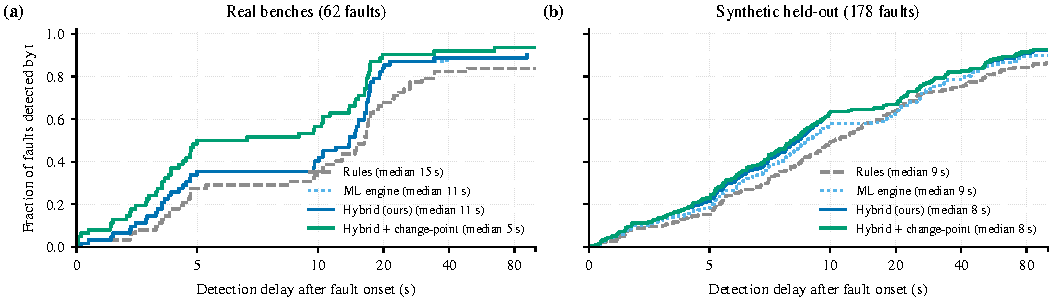
\includegraphics[width=\textwidth]{fig_delay.pdf}
\caption[Detection delay after fault onset as a cumulative distribution]{Detection delay after fault onset as a cumulative distribution (symmetric-log axis); legends give the median over detected faults. The curves plateau at each engine's detection rate.}
\label{fig:delay}
\end{figure}

\subsection{Ablation}
\label{sec:ablation}
Figure~\ref{fig:abl} removes one mechanism of the corrected ML engine at a time. The most important single component is still the \code{docker stop} fact: without it \cn{} falls by 18 points on the real systems and 15 on the synthetic set, because every stopped service goes unnamed. The crash-loop fact (0 and 7 points) and the random walk (3 and 2 points) each contribute. Two mechanisms act on the contract rather than on accuracy. Without the load factor nothing changes on injected faults (the load does not move in them) and the effect appears only on the workload recordings of Section~\ref{sec:workloadres}: false alarms rise from 0.0 to 1.2 and from 1.0 to 1.9 per hour there. With the MAD spread instead of the tail-aware one, alarm time on the real systems doubles (6\% to 12\%) and, on the workload recordings, rises from 0\% to 10\% and 6\% (13\% and 31\% when the load factor is also removed). Removing the one-sided features raises alarm time on the real systems from 6\% to 24\%; the two-speed drift keeps it at 6\% instead of 13\% and false alarms at 2.3 instead of 3.1 per hour. Alarming at level one instead of two raises \cn{} by 2 points on both sets but more than doubles the false alarms on the real systems (5.4 per hour). The one-sided features do not matter on the synthetic set, where restarts do not lower memory: an effect of the real systems that the simulator does not reproduce. The range guard of the first version has no counterpart: the robust spread takes its place.

\begin{figure}[!htbp]
\centering
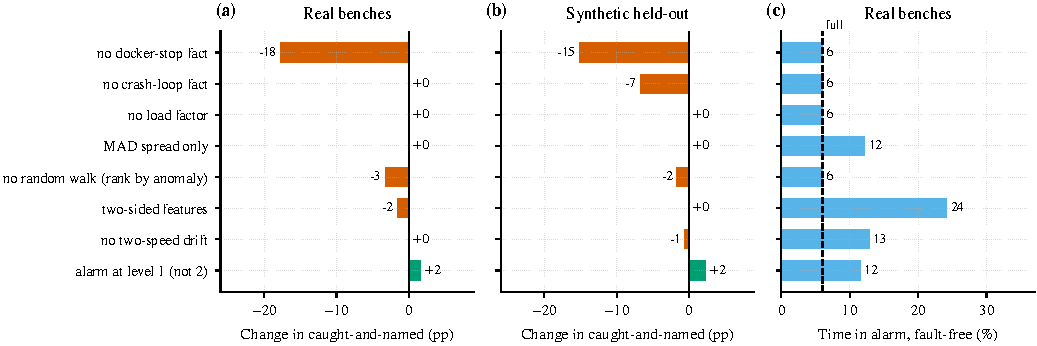
\includegraphics[width=\textwidth]{fig_ablation.pdf}
\caption[Ablation. Each bar removes one mechanism from the full engine.]{Ablation of the corrected ML engine. Each bar removes one mechanism from the full engine. (a), (b): change in caught-and-named rate (percentage points) on the real systems and the synthetic held-out set. (c): share of fault-free time in alarm on the real systems; the dashed line marks the full engine.}
\label{fig:abl}
\end{figure}

\subsection{When does the graph matter? The amplification study}
Standard benchmarks have faults whose own service is also the loudest, which is the case where ranking by severity cannot fail. To probe the regime in which it can, soft faults (brownout, latency, memory) were regenerated with the amplification factor $A \in \{1, 1.5, 2, 3, 4\}$, the hybrid's alarms were kept identical for every ranker, and only the ranking varied (Figure~\ref{fig:amp}). As $A$ grows, the share of faults in which some victim is louder than the true cause rises from 10\% to 21\% (panel c), the severity ranking falls from 76\% to 71\%, and the walk holds at 75 to 76\%. The gain of the walk over severity therefore grows from zero to $+3.8$ points (95\% CI $[-0.9, +9.4]$ at $A = 4$) and that of the walk with learned directions to $+4.7$ ($[-0.9, +10.4]$) (panel b). The intervals include zero at every level. In the first version of the study the own-versus-explained decomposition of the rule layer was the strongest ranker on soft faults; with the corrected ML engine it is not (71 to 75\%, $-1.9$ to $0.0$ points against severity, intervals including zero), because the engine's own and symptom levels now carry the same separation. A router that uses it whenever no container fact holds did not change the full benchmarks (within $\pm 2$ points), so the shipped ranking is unchanged. Graph-aware ranking remains a modest, regime-dependent gain that this sample is too small to confirm.

\begin{figure}[!htbp]
\centering
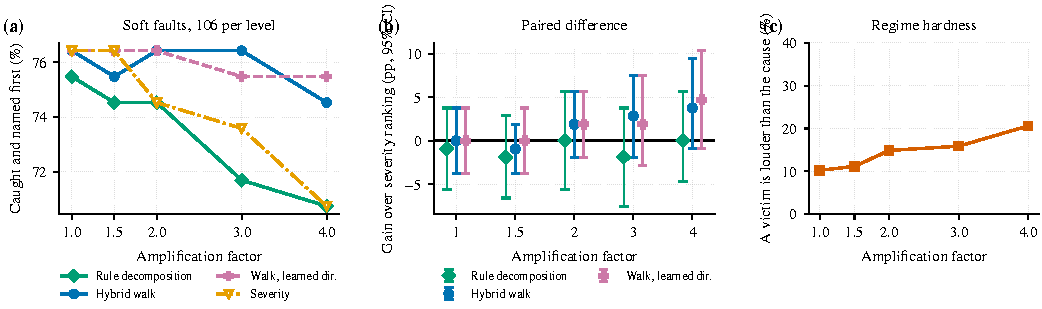
\includegraphics[width=\textwidth]{fig_amp.pdf}
\caption[Amplification study on soft faults (106 per level)]{Amplification study on soft faults (106 per level). (a) Caught-and-named rate of four rankers on identical alarms. (b) Gain over the severity ranking with 95\% paired-bootstrap intervals. (c) Share of faults in which a victim is louder than the true cause.}
\label{fig:amp}
\end{figure}

\subsection{The cascade model}
Figure~\ref{fig:cal} evaluates who-is-next predictions at the first alarm of each fault: for every service still healthy, the probability that it turns unhealthy before the fault ends. On the synthetic set (163 faults, 1\,289 predictions, 69 cascades) the learned propagation model reaches AUROC 0.841 against 0.827 for the same noisy-OR with every edge fixed at 0.7, a Brier score of 0.047 against 0.052 and an ECE of 0.033 against 0.051. The calibration is better than that of the fixed model, the ranking only slightly. The reliability curve is noisy in the upper bins, which hold few predictions. \emph{On the real systems the experiment cannot be done well:} only 10 of 535 predictions were followed by a cascade (56 faults), so the real-system comparison (AUROC 0.742 against 0.633; the live mapper's own risk values 0.591) is not informative. The real faults are mostly single-service outages that the systems absorb; whether learned propagation helps on a real cascade is untested.

\begin{figure}[!htbp]
\centering
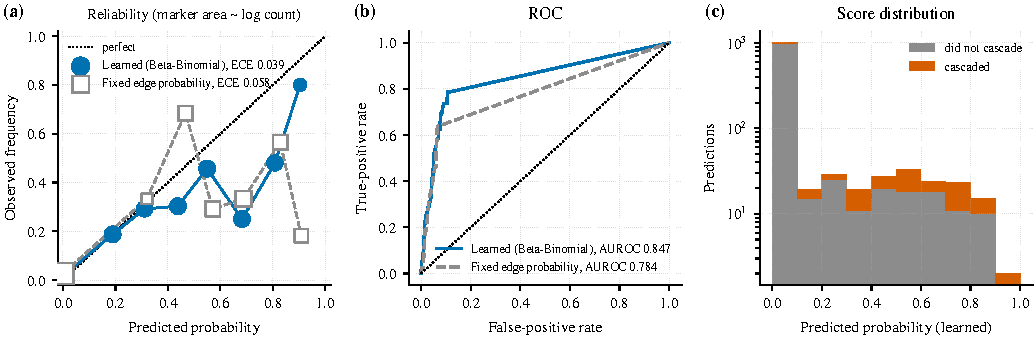
\includegraphics[width=\textwidth]{fig_calibration.pdf}
\caption[Who-is-next prediction on the synthetic held-out set]{Who-is-next prediction on the synthetic held-out set. (a) Reliability diagram with equal-width bins and marker area proportional to the logarithm of the bin count. (b) ROC curves. (c) Distribution of the learned predicted probabilities.}
\label{fig:cal}
\end{figure}

\subsection{Learned directions}
Figure~\ref{fig:dirs} reports direction accuracy on observed pairs that are true calls. With names available the name rule is correct for 21 of 31 real pairs (and leaves 10 undecided); the learned rule is correct for 27 of 31 (4 wrong). With service names hidden the name rule is undecided for every pair while the learned rule is unchanged; the same holds on the synthetic set (95 of 204 against 198 of 204 correct). The effect on ranking is smaller than The effect on directions. With names available the learned directions do \emph{not} beat the name rule (68\% against 71\% on the real systems, $-3.2$ points, not significant). With names hidden they reach 68\% against 66\% for the name rule and 71\% for the true graph. Learned directions are a robustness mechanism, not an accuracy gain.

\begin{figure}[!htbp]
\centering
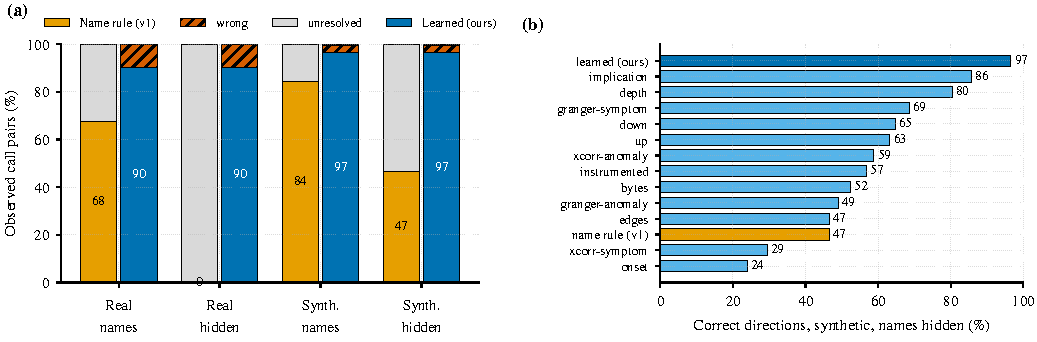
\includegraphics[width=\textwidth]{fig_dirs.pdf}
\caption[Call directions: name rule against learned rule]{Call directions. (a) Share of observed true-call pairs oriented correctly, wrongly, or left unresolved by the name rule and by the learned rule, with service names shown or hidden. (b) Correct share of each individual signal on the synthetic set with names hidden.}
\label{fig:dirs}
\end{figure}

\subsection{Early warning and fault diagnosis}
The trend forecast (now a straight line through the recent deviations from what the load predicts) warns before the alarm for 13 of 178 synthetic faults (7 of 18 memory leaks, 4 of 25 latency faults, 2 of 26 brownouts) with a median lead of 25\,s and 0.8 false warning episodes per fault-free hour (Figure~\ref{fig:early}); the first version, on the raw readings, warned for 16 (5 of 26 brownouts). On the real systems it fired before the alarm for none of the 62 faults, since those faults are abrupt, and raised 6.9 false warning episodes per hour; early warning of gradual faults is the weakest part of the system and is reported as such. Figure~\ref{fig:diag} shows fault-type diagnosis. With the true service the forest is correct for 99\% of synthetic faults 60\,s after the alarm; on the engine's own suspect it is 79\%, because a wrong suspect is rarely typed correctly. On the real systems a hand-written decision list generalises best (64\% on the suspect, 84\% on the true service), because real flaps are pause cycles and real brownouts on idle services show no throttling: differences between the simulator and the real systems that the learned models absorb as synthetic-specific patterns.

\begin{figure}[!htbp]
\centering
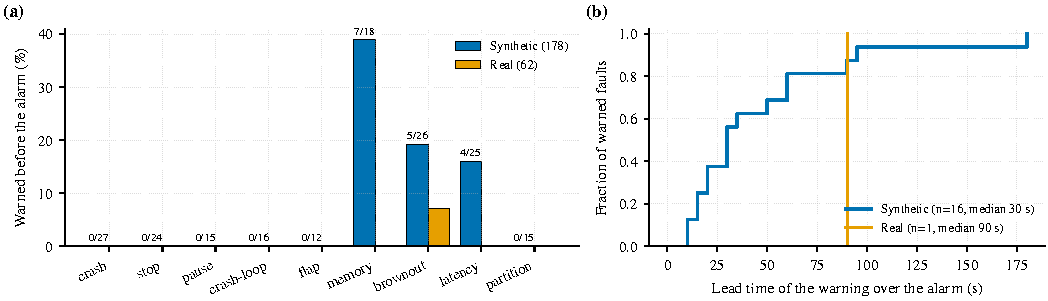
\includegraphics[width=\textwidth]{fig_early.pdf}
\caption[Early warning by fault class and lead time]{Early warning. (a) Share of faults warned before the alarm, by fault class. (b) Lead time of the warnings over the alarm as a cumulative distribution.}
\label{fig:early}
\end{figure}

\begin{figure}[!htbp]
\centering
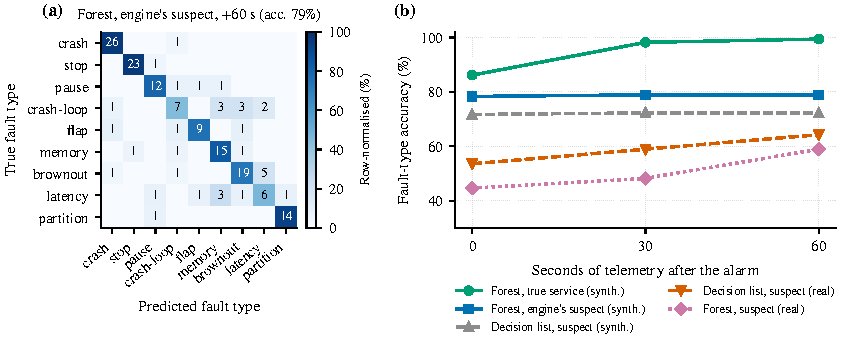
\includegraphics[width=\textwidth]{fig_diag.pdf}
\caption[Fault-type diagnosis]{Fault-type diagnosis. (a) Confusion matrix (counts; shading is row-normalised) of the random forest on the engine's suspect 60\,s after the alarm, synthetic held-out set. (b) Accuracy against seconds of telemetry after the alarm, for the true service and the engine's suspect.}
\label{fig:diag}
\end{figure}

\subsection{Cost}
\label{sec:cost}
The pipeline is unsupervised, needs no GPU and runs on one core. Figure~\ref{fig:scale} times one complete decision window (container facts, the model of normal, random walk, forecast) on random call graphs of 10 to 320 services, after a warm-up long enough for every service to have a model. The adopted load-aware model costs about $0.37$\,ms per service per window and grows linearly: 4.0\,ms for 10 services, 26.8\,ms for 80 and 119\,ms for 320 (95th percentile 356\,ms), always far below the 5\,s collection period. The old forest cost about $0.9$\,ms per service (296\,ms for 320) with 95th-percentile windows nine times the mean, because every service refits at once every ten readings. The load-aware model refreshes its baselines every four readings with a much smaller peak (about three times the mean). The subspace residual grows faster than linearly (1.2\,s for 320 services, with 11\,s windows at the 95th percentile) because its covariance has one row per service-signal pair. On the two benches (12 and 13 services) a window takes about 5\,ms. These are wall-clock times on one core of a shared four-core virtual machine, not a tuned benchmark.

\begin{figure}[!htbp]
\centering
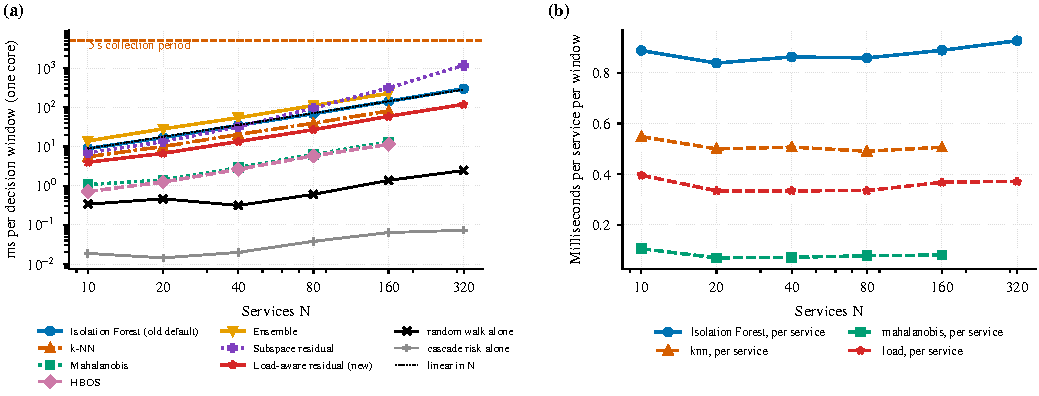
\includegraphics[width=\textwidth]{fig_scale.pdf}
\caption[Cost of one decision window against the number of services]{Cost of one decision window against the number of services (single core, logarithmic axes; the dashed line is the 5\,s collection period). (a) Mean milliseconds per window for each model of normal, the random walk and the cascade risk alone. (b) Milliseconds per service per window.}
\label{fig:scale}
\end{figure}

\subsection{Case studies}
Figure~\ref{fig:case} shows three real incidents, chosen by class before looking at the outcome. In (a) a memory leak overlaps several outages: the engine names the stopped containers first, as it should, and only a model of concurrent faults could do better. In (b) a crash loop is named correctly about 30\,s after its first kill and stays named between kills. In (c) a brownout on an almost idle service never raises an alarm, which is the open problem of Figure~\ref{fig:class}.

\begin{figure}[!htbp]
\centering
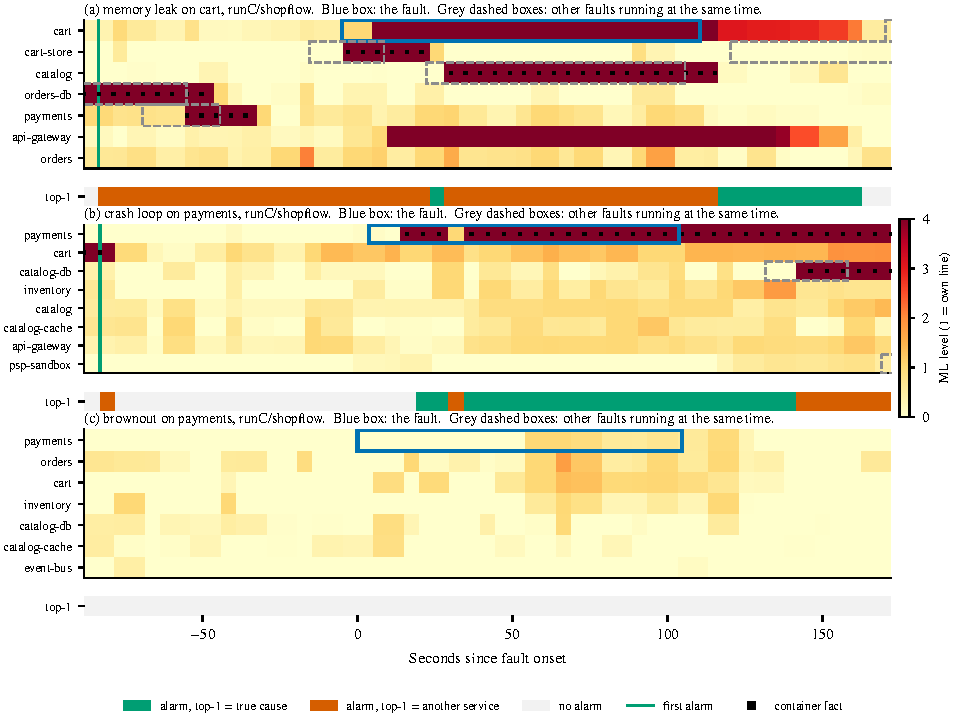
\includegraphics[width=0.86\textwidth]{fig_case.pdf}
\caption[Three real incidents]{Three real incidents. Heat maps show the ML level of the most relevant services; the blue box is the fault, grey dashed boxes are other faults running at the same time, black squares mark container facts, the green line is the first alarm in the window (an alarm already ongoing from an earlier fault starts at the left edge), and the strip below each map shows whether the engine's top-ranked service was the true cause.}
\label{fig:case}
\end{figure}

\subsection{The three engines on one live fault}
\label{sec:engineslive}
To show what the Detection engines page adds, the simulator was run with a slow \texttt{payment} service (CPU saturated at 97\% from second 30 of the fault run; \texttt{orders} follows at 86\% twelve seconds later), the ground-truth root cause being \texttt{payment}. The three engines were read every four seconds through the page's API after a 260-second quiet period (Table~\ref{tab:live}).
\begin{table}[!htbp]
\centering
\caption[One simulated fault: each engine's first suspect over time]{One simulated fault (slow \texttt{payment}): each engine's first suspect and its peak against its own alarm line, at three moments after the onset. The simulator reports every two seconds, so 24 readings are 48 s here (two minutes on a real host).}
\label{tab:live}
\footnotesize
\renewcommand{\arraystretch}{1.2}
\begin{tabular}{l>{\raggedright\arraybackslash}p{0.22\textwidth}>{\raggedright\arraybackslash}p{0.3\textwidth}>{\raggedright\arraybackslash}p{0.22\textwidth}}
\toprule
\textbf{Engine} & \textbf{+5 s: payment only} & \textbf{+20 to +70 s: both saturated} & \textbf{after +75 s}\\
\midrule
Rules & payment (3.0$\times$) & orders (3.7$\times$), payment second (3.0$\times$) & the same\\
ML & payment (88\% of the walk), peak 1.3 & payment (57\%), orders (43\%), peak 1.3 & absorbed: no alarm\\
Hybrid & payment & payment (0.91), orders (0.87) & orders (alarm kept by the rules)\\
\bottomrule
\end{tabular}
\end{table}
This is one simulated fault and an illustration, not evidence. It shows the mechanism the evaluation measures at scale: the rule layer ranks the loudest service first, so it blames \texttt{orders} as soon as both are saturated, while the ML engine lets the walk keep the blame on the source. It also shows the price of the two-minute drift rule (Section~\ref{sec:whichmodel}): a saturation that lasts longer than the acceptance time is absorbed as the new normal and the ML alarm clears. The hybrid keeps alarming because of the rule layer, but its ranking then follows the rules.

\subsection{Operational findings from the benchmark hosts}
\label{sec:hostfindings}
Operating the benchmark hosts produced three findings that changed the tools.
\begin{itemize}
\item A host too small for its workload looks like a mapper fault. The OpenTelemetry demo ran on a 2-vCPU, 4 GiB instance, with a load average of about 25 and 3.6 of 3.8 GiB of memory in use, no swap, and Docker did not answer within 25 seconds; the dashboard showed no services. A second host with 4 GiB of swap and a load average of 0.2 ran 27 containers of a social-network benchmark normally. The lesson is operational: the mapper depends on the host's Docker daemon answering, and a host that cannot answer shows nothing. The check tool now says so in one step.
\item Idle front ends have no edges. On a healthy social-network host, the front-end containers showed no outgoing sockets when sampled, because nothing was calling them; an undeclared edge expires ten minutes after its last traffic. A front end that is idle therefore has no edge until traffic arrives, which is correct behaviour but looks like a fault. Declared edges from the Compose file keep an idle link on the screen.
\item Hard-coded project names blocked traffic; the traffic controller accepted only five named projects, so benchmark hosts with other names could not be driven. Unknown projects now get a generic workflow.
\end{itemize}


\section{Live Fault Lab Experiments: Auto-restart On and Off}
\label{sec:live}
The 62-fault evaluation above was made on recorded campaigns. To test the mapper once more against a system it cannot see into, and to settle whether its optional auto-restart changes the results, both benchmark benches (Section~\ref{sec:benches}) were run live inside Docker, reached by the mapper over SSH exactly like a remote host (auto-restart exists only on that path). The Fault Lab replayed the \emph{same} plan every time (seed 11, the \texttt{stormy} profile, crash, stop, pause and brownout faults, 18 minutes, 21 faults), once with \texttt{MAPPER\_AUTO\_RESTART} on and once with it off, after a 6-minute warm-up. The hybrid engine decided the incidents and the harness scored them against the injector's private ledger. Only one bench ran at a time. The run scripts and every recorded file are in the repository (\texttt{run/scripts/autorestart-experiment.sh}, \texttt{run/recorded-runs/autorestart/}).

\begin{table}[!htbp]
\centering
\caption{Live campaigns, same fault plan, auto-restart on and off (21 faults each; 95\% Wilson intervals).}
\label{tab:livecampaign}
\small
\renewcommand{\arraystretch}{1.2}
\begin{tabular}{llrrrrr}
\toprule
\textbf{Bench} & \textbf{Auto-restart} & \textbf{Detected} & \textbf{Top-1 (\%)} & \textbf{Top-3 (\%)} & \textbf{Delay (s)} & \textbf{FA/h}\\
\midrule
ShopFlow & on  & 100\% & 33 [17, 55] & 71 [50, 86] & 3.3 & 9.2\\
ShopFlow & off & 100\% & 24 [11, 45] & 71 [50, 86] & 2.6 & 0.0\\
LedgerLine & on  & 95\% & 55 [34, 74] & 65 [43, 82] & 9.7 & 0.0\\
LedgerLine & off & 95\% & 40 [22, 61] & 70 [48, 85] & 3.9 & 3.1\\
\bottomrule
\end{tabular}

\smallskip
{\footnotesize Delay is the median time from fault onset to the first alarm; FA/h is false-alarm episodes per fault-free hour.}
\end{table}

\begin{table}[!htbp]
\centering
\caption{Top-1 and Top-3 root-cause accuracy (\%) by fault class in the live campaigns (on / off).}
\label{tab:liveclass}
\small
\renewcommand{\arraystretch}{1.15}
\begin{tabular}{lrrrr}
\toprule
 & & & \textbf{ShopFlow} & \textbf{LedgerLine}\\
\textbf{Fault class} & \textbf{Faults} & & \textbf{Top-1 / Top-3} & \textbf{Top-1 / Top-3}\\
\midrule
Brownout & 6 & on / off & 0 / 17 \hspace{4pt} 0 / 0 & 0 / 0 \hspace{4pt} 0 / 20\\
Crash & 6 & on / off & 33 / 83 \hspace{4pt} 33 / 100 & 80 / 80 \hspace{4pt} 33 / 83\\
Pause & 7 & on / off & 57 / 100 \hspace{4pt} 29 / 100 & 86 / 100 \hspace{4pt} 86 / 100\\
Stop & 2 & on / off & 50 / 100 \hspace{4pt} 50 / 100 & 50 / 100 \hspace{4pt} 0 / 50\\
\bottomrule
\end{tabular}
\end{table}

\textbf{What the numbers show.} Every fault but one was detected in both systems, and the true cause was within the top three suspects in 65 to 71\,\% of the faults. The differences between the on and off rows are 9 and 15 points of Top-1, and the false-alarm column moves in opposite directions (more with auto-restart on in ShopFlow, fewer in LedgerLine). With 21 faults the intervals overlap completely, so none of these differences can be called an effect of auto-restart. Brownouts are the weak class in all four runs (no Top-1 at all), which agrees with the 62-fault results of Section~\ref{sec:resultsmain}.

\textbf{Why there was no effect to find.} The log of each run shows what auto-restart actually did. It restarted no container of the bench under test. The one restart in each ``on'' run was of the \emph{other} bench's message bus, which had been stopped by hand to keep one bench per run and which exited with code 1; the mapper, which sees every container on the host, restarted it. That is an artefact of the setup and is reported as such. Three properties of the mapper and the benches explain the rest:
\begin{itemize}
\item the benches set \texttt{restart: always}, so Docker brings a crashed container back within seconds, before the mapper's next pass;
\item the mapper only looks for dead containers once per discovery cycle (180\,s), longer than the 20-second crash faults;
\item it skips containers that exited with code 0, and a container stopped with \texttt{docker stop} exits with code 0.
\end{itemize}

\begin{sloppypar}
\textbf{A direct test with long outages.} To give auto-restart a chance to act, \texttt{cart} and \texttt{payments} were each stopped for 5 minutes by the Fault Lab (\texttt{run/scripts/autorestart-stop-test.sh}), with the state of each container sampled every 2 seconds. Table~\ref{tab:stoptest} shows no difference: the mapper left the containers down in both modes.
\end{sloppypar}

\begin{table}[!htbp]
\centering
\caption{Time a stopped container stayed down, with auto-restart on and off (injector releases it after 300\,s).}
\label{tab:stoptest}
\small
\begin{tabular}{lrr}
\toprule
\textbf{Container} & \textbf{On (s)} & \textbf{Off (s)}\\
\midrule
cart & 299 & 298\\
payments & 301 & 301\\
\bottomrule
\end{tabular}
\end{table}

\textbf{Conclusion.} On these benchmarks auto-restart is inert: it neither helped nor hurt detection or root-cause accuracy beyond run-to-run variation, and the rule that skips exit code 0 means a deliberate stop is never undone. It would matter on a host whose containers have no restart policy and exit with a failure code, which these benches do not model, so that case is untested. Switching it off for evaluation remains the safe default, because the mapper then cannot heal what the injector breaks.

\section{Analysis}
\textbf{What the evidence supports.} The first ML engine mistook a change of workload for a fault: on fault-free recordings it sat in alarm for 23 to 52\% of the time, and every workload-blind detector we tried did the same or worse (Section~\ref{sec:workloadres}). The load-aware model that replaced it stays quiet on both recordings and loses nothing on injected faults. Container facts carry more weight than any other component; the ablation costs 18 and 15 points when the \code{docker stop} fact goes. And learned propagation calibrates better than fixed edge probabilities on observed cascades (ECE 0.033 against 0.051, AUROC 0.841 against 0.827).

\textbf{What did not work.} Several expected gains never appeared. The corrected engine is no more accurate than the first on injected faults. Hybrid over rules was significant in the first version ($+9.7$ points, $p = 0.032$) and is not now ($+8.1$, $p = 0.117$), so the improvement sits in robustness, not in the benchmark score. The random walk does not beat ranking by anomaly alone, learned directions do not beat the name rule when names exist, and onset-precedence re-ranking changed nothing. The subspace residual, the principled multivariate alternative, discriminates as well as the adopted model but raises more false alarms on the load steps and costs more. We report these because an operator gains more from a pipeline that states where it stops. The plain rule $z$-score remains a strong detector. The load-aware model earns its place by staying quiet under changing load and by catching faults the rules miss, not by separating faulted services better.

\textbf{The measurement bugs.} Before we fixed the ledger reader, every engine scored against only part of the real faults (14 of 31 per system stayed hidden), and the outages of the hidden faults counted as false alarms. Every number in this report therefore uses all 62 faults, and a regression test guards the reader. A second bug in the replay (Section~\ref{sec:bug2}) deleted the idle stretches from the recordings. That bug explains why the benchmarks never exposed the first ML engine's failure; an operator found it on a live system. Both bugs flattered the engines.

\section{Discussion and Threats to Validity}
\textbf{Construct validity.} The injector's ledger is the ground truth. It names the structural root cause and the services able to suffer. Whether a service visibly suffers depends on protections the ledger does not model, so cascade recall understates true propagation. The offline recordings keep no edge evidence, which leaves the evidence weighting of Section~\ref{sec:graph} unmeasured.

\textbf{Internal validity.} The authors chose the settings. We swept the alarm line, window and slow reference of the load-aware model over all recordings together (Figure~\ref{fig:zline}), which amounts to tuning on test data; the adopted values sit in the sweep's flat region, not at its maximum. On the synthetic track a disjoint tuning split picked the settings and the test split was scored once. On the real track no held-out system exists, so the real numbers run optimistic by an unknown margin. We found the two container facts by inspecting the real runs.

\textbf{External validity.} Two real applications, one capture and live recordings on one machine limit the claim. Generators produced the workload recordings (organic or closed-loop), so a real day of users stays untested, and a fault that begins during a large change of load can hide behind the load-aware model. Architecture independence rests on the cross-system check and on synthetic topologies. It is argued, not proven. The simulator is also cleaner than a real system: restarts do not lower memory in it.

\textbf{Conclusion validity.} With 62 real faults, no difference below about ten points is resolvable, and overlapping faults make the intervals optimistic. The workload claims rest on four fault-free recordings of 62 and 72 minutes. The effect is large (0\% against 23 to 96\% of the time in alarm), but four recordings are few.

\textbf{Auto-restart.} The mapper can restart crashed containers on a target (Section~\ref{sec:tools}, Chapter~\ref{ch:system}). Live campaigns with the feature on and off showed no effect on these benches (Section~\ref{sec:live}). Even so, switch it off for evaluation runs so the mapper cannot heal the faults the injector applies.

\section{Comparison with Existing Approaches}
The published methods in Table~\ref{tab:litreview} were not re-implemented on our recordings, so there is no head-to-head accuracy table against them. What is compared head to head are the baselines that those methods build on: the rule layer, ranking by anomaly alone (the severity ranking), the walk, and the ML engine in its two versions. Table~\ref{tab:vsexisting} sets the measured results beside the qualitative properties of Chapter~\ref{ch:lit}.

\begin{table}[!htbp]
\centering
\caption{This project beside the approaches it builds on. Accuracy figures are caught-and-named on the 62 real faults.}
\label{tab:vsexisting}
\small
\renewcommand{\arraystretch}{1.25}
\begin{tabularx}{\textwidth}{>{\raggedright\arraybackslash}p{3.7cm}>{\raggedright\arraybackslash}p{2.0cm}>{\raggedright\arraybackslash}X}
\toprule
\textbf{Approach} & \textbf{C+N (real)} & \textbf{Notes}\\
\midrule
Rule layer (z-score) & 63\% & Fast, 9 false-alarm episodes per hour, 9\% alarm time\\
Severity ranking (loudest service) & 68\% & Cannot fail when the cause is loudest; weakens as victims get louder\\
Per-service Isolation Forest + walk (first version) & 69\% & 4.6 false alarms per hour; in alarm for 23 to 52\% of the time when only the load moves\\
ML engine (load-aware model + walk) & 71\% & Fewest false alarms (2.3 per hour), 6\% alarm time; 0\% when only the load moves\\
\textbf{Hybrid (this project)} & \textbf{71\%} & Paired $+8.1$ points over rules (not significant); names stops 16 of 16\\
Learned fusion methods \cite{zhang2023diagfusion,sun2024deephunt,lee2023eadro} & not run & Need labelled failures and GPU; not auditable\\
Trace-based rankers \cite{yu2021microrank} & not run & Need tracing in every service\\
\bottomrule
\end{tabularx}
\end{table}

\section{Significance and Implications}
An instrumentation-free tool can recover a usable call graph and a useful ranking, and for small teams that is the difference between having a diagnosis tool and not. Container facts are worth more than any statistical refinement: a stopped container is something one knows, and folding it into an anomaly score throws information away. And the right operating contract for an alarm is the one the operator experiences, which is why alarm time is reported beside false-alarm episodes.
